\documentclass[10pt]{article}
% Math Packages
\usepackage{amsmath, mathtools}
\usepackage{amssymb}
\usepackage{amsthm}
\usepackage{amsfonts}
\usepackage{bbm}
\usepackage{breqn}
\usepackage[margin=1in]{geometry}
\usepackage{graphicx}
\usepackage{tikz}
\usetikzlibrary{arrows.meta}
\usetikzlibrary{calc}
\usepackage{forest}
\usepackage{tikz-qtree}
\graphicspath{ {./images/} }
\usepackage{hyperref}
\usepackage[capitalize]{cleveref}
\usepackage[shortlabels]{enumitem}
\usetikzlibrary{arrows,matrix,positioning}
\usepackage{multicol}

% for the pipe symbol
\usepackage[T1]{fontenc}

% Citing theorems by name. (source: https://tex.stackexchange.com/questions/109843/cleveref-and-named-theorems)
\makeatletter
\newcommand{\ncref}[1]{\cref{#1}\mynameref{#1}{\csname r@#1\endcsname}}

\def\mynameref#1#2{%
  \begingroup
  \edef\@mytxt{#2}%
  \edef\@mytst{\expandafter\@thirdoffive\@mytxt}%
  \ifx\@mytst\empty\else
  \space(\nameref{#1})\fi
  \endgroup
}
\makeatother

% Colorful Notes
\usepackage{color} \definecolor{Red}{rgb}{1,0,0} \definecolor{Blue}{rgb}{0,0,1}
\definecolor{Purple}{rgb}{.5,0,.5} \def\red{\color{Red}} \def\blue{\color{Blue}}
\def\gray{\color{gray}} \def\purple{\color{Purple}}
\newcommand{\rnote}[1]{{\red [#1]}} % \rnote{foo} gives '[foo]' in red
\newcommand{\pnote}[1]{{\purple [#1]}} % \pnote{foo} gives '[foo]' in purple
\newcommand{\bnote}[1]{{\blue #1}} % \bnote{foo} gives 'foo' in blue
\newcommand{\gnote}[1]{{\gray #1}} % \gnote{foo} gives 'foo' in gray
\newcommand{\Max}[1]{{\purple [#1]}} % \bnote{foo} then 'foo' is blue


% Claim numbering (the counter restarts after each proof environment)
\newcounter{claimcount}
\setcounter{claimcount}{0}
\newenvironment{claim}{\refstepcounter{claimcount}\par\addvspace{\medskipamount}\noindent\textbf{Claim \arabic{claimcount}:}}{}
\usepackage{etoolbox}
\AtBeginEnvironment{proof}{\setcounter{claimcount}{0}}
\newenvironment{claimproof}{\par\addvspace{\medskipamount}\noindent\textit{Proof of Claim  \arabic{claimcount}.}}{\hfill\ensuremath{\qedsymbol} \tiny{Claim}

  \medskip}
% Add claim support to cleverref
\crefname{claimcount}{Claim}{Claims}


% Math Environments
\newtheorem{theorem}{Theorem}
\newtheorem{assumption}[theorem]{Assumption}
\newtheorem{lemma}[theorem]{Lemma}
\newtheorem{proposition}[theorem]{Proposition}
\newtheorem{corollary}[theorem]{Corollary}
\newtheorem{question}[theorem]{Question}
\theoremstyle{definition}
\newtheorem{definition}[theorem]{Definition}
\newtheorem{remark}[theorem]{Remark}
\newtheorem{example}[theorem]{Example}
\newtheorem{notation}[theorem]{Notation}
\newtheorem{problem}[theorem]{Problem}

% Matrices and Column Vectors. 
\usepackage{stackengine}
\setstackgap{L}{1.0\normalbaselineskip}
\usepackage{tabstackengine}
\setstackEOL{;}% row separator
\setstackTAB{,}% column separator
\setstacktabbedgap{1ex}% inter-column gap
\setstackgap{L}{1.5\normalbaselineskip}% inter-row baselineskip
\let\nmatrix\bracketMatrixstack  %Usage: \nmatrix{1,2,3\4,5,6}
\newcommand\cv[1]{\setstackEOL{,}\bracketMatrixstack{#1}} %usage: \cv{1,2,3}

% Custom Math Coqmmands
\newcommand{\vt}{\vskip 5mm} % vertical space
\newcommand{\fl}{\noindent\textbf} % first line
\newcommand{\Fl}{\vt\noindent\textbf} % first line with space above
\newcommand{\norm}[1]{\left\lVert#1\right\rVert} % norm
\newcommand{\pnorm}[1]{\left\lVert#1\right\rVert_p} % p-norm
\newcommand{\qnorm}[1]{\left\lVert#1\right\rVert_q} % q-norm
\newcommand{\1}[1]{\textbf{1}_{\left[#1\right]}} % indicator function 
\def\limn{\lim_{n\to\infty}} % shortcut for lim as n-> infinity
\def\sumn{\sum_{n=1}^{\infty}} % shortcut for sum from n=1 to infinity
\def\sumkn{\sum_{k=1}^{n}} % shortcut for sum from k=1 to n
\def\sumin{\sum_{i=1}^{n}} % shortcut for sum from i=1 to n
\def\SAs{\sigma\text{-algebras}} % shortcut for $\sigma$-algebras
\def\SA{\sigma\text{-algebra}} % shortcut for $\sigma$-algebra
\def\Ft{\mathcal{F}_t} % time-indexed sigma-algebra (t)
\def\Fs{\mathcal{F}_s} % time-indexed sigma-algebra (s)
\def\F{\mathcal{F}} % sigma-algebra
\def\G{\mathcal{G}} % sigma-algebra
\def\R{\mathbb{R}} % Real numbers
\def\N{\mathbb{N}} % Natural numbers
\def\Z{\mathbb{Z}} % Integers
\def\E{\mathbb{E}} % Expectation
\def\P{\mathbb{P}} % Probability
\def\Q{\mathbb{Q}} % Q probability
\def\dist{\text{dist}} %Text 'dist' for things like 'dist(x,y)'
\newcommand{\indep}{\perp \!\!\! \perp}  %independence symbol
\def\Var{\mathrm{Var}} % Variance
\def\tr{\mathrm{tr}} % trace

% Brackets and Parentheses
\def\[{\left [}
    \def\]{\right ]}
% \def\({\left (}
%   \def\){\right )}



\usepackage{color}
\definecolor{Red}{rgb}{1,0,0}
\definecolor{Blue}{rgb}{0,0,1}
\definecolor{Purple}{rgb}{.5,0,.5}
\def\red{\color{Red}}
\def\blue{\color{Blue}}
\def\gray{\color{gray}}
\def\purple{\color{Purple}}
\definecolor{RoyalBlue}{cmyk}{1, 0.50, 0, 0}
\newcommand{\dempfcolor}[1]{{\color{RoyalBlue}#1}} 
\newcommand{\demph}[1]{\dempfcolor{{\sl #1}}}

% comment exactly one of the following line to show / hide the solutions
% \newcommand{\solution}[1]{{\purple #1}} % uncomment to show the solutions
\newcommand{\solution}[1]{} % uncomment to hide the solutions



\title{Lecture Notes for Math 372: \\Elementary Probability and Statistics}
\date{Last updated: \today}
% \author{mh}

\begin{document}
\begin{center}
  \section*{Math 372: Practice Midterm 2}
\end{center}

\begin{problem}
  An evil sorcerer decides to summon some minions to help clean up his lawn
  after a big storm. His magic spell summons up to 2 skeletons and up to 2
  abyssal specters. Let $X$ be the number of skeletons summoned, and let $Y$
  be the number of abyssal specters summoned. According to the notes in his
  spellbook, the joint pmf of $X$ and $Y$ is given by:
  \begin{equation*}
    \begin{array}{c|ccc}
      p(x,y) & y=0 & y=1 & y=2 \\ \hline
      x=0 & 0.12 & 0.10 & 0.08 \\
      x=1 & 0.06 & 0.18 & 0.14 \\
      x=2 & 0.04 & 0.08 & 0.20 \\
    \end{array}
  \end{equation*}

  \begin{enumerate}[(a)]
    \item What is the probability that the necromancer summons an even number
    of minions?
    \item Compute $\P[X \leq 1 \text{ and } Y \leq 1]$.
    \item Using words, describe the event $[X+Y\geq 2]$, and then compute its
    probability.
    \item Compute the marginal pmf of $X$ and $Y$. Using $p_X(x)$, find $\P[X \ge 1]$.
    \item Are $X$ and $Y$ independent? Justify your answer.
  \end{enumerate}
\end{problem}



\begin{problem}%[normal - 4.3.45]
  A machine that produces ball bearings has initially been set so that the
  true average diameter of the bearings it produces is $.500$ cm. A bearing is
  acceptable if its diameter is within $.004$ cm. of this target value.
  Suppose, however, that the setting has changed during the course of
  production, so that the bearings have normally distributed diameters with
  mean value $.499$ cm. and standard deviation $.002$ cm. What percentage of
  the bearings produced will not be acceptable? [Hint: use the following plot
  of the standard normal density curve.]

  \begin{center}
    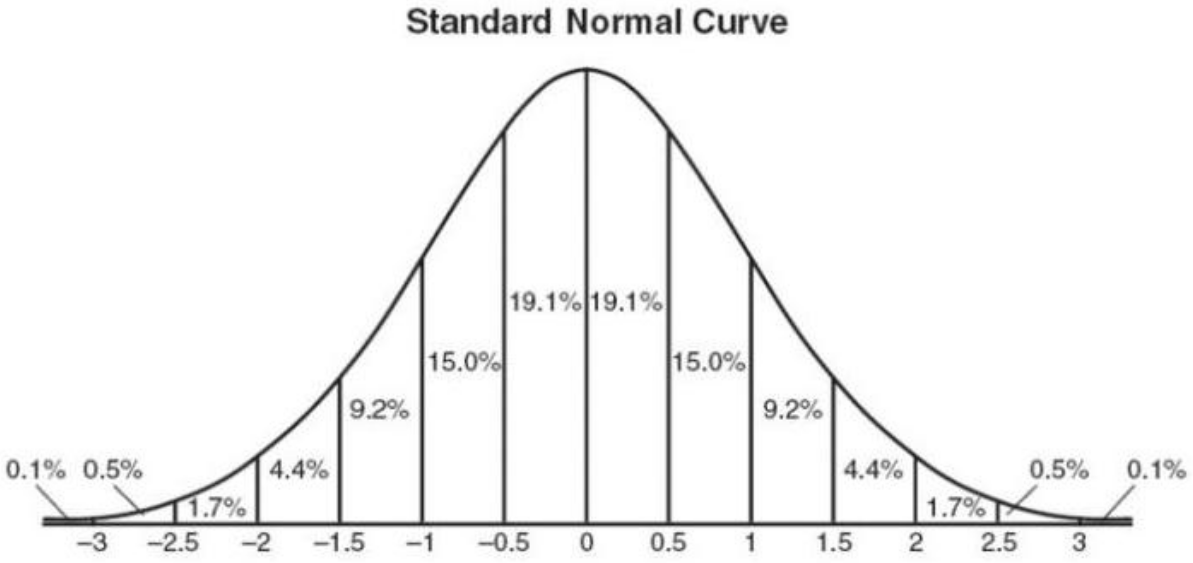
\includegraphics[scale=.34]{images/standard-normal-small.png}
  \end{center}
\end{problem}





\begin{problem}
  Fix $\beta>0$, and let $X$ be a random variable with cdf
  \begin{equation*}
    F(t) = \left\{ \begin{array}{l@{\quad:\quad}l} 1- \left( \frac{\beta}{t} \right)^{3}  & t \geq \beta\\ 0& t<\beta\end{array}\right.
  \end{equation*}
  \begin{enumerate}[(a)]
    \item Find $f$, the pdf of $X$.
    \item Find $\E\left[X \right]$.
    \item Find $\P\left[\beta \leq X \leq 2\beta\right]$.
  \end{enumerate}
\end{problem}


\begin{problem}%[continuous rv]
  Let $T$ be the time, in minutes, between successive drink orders at a bar. Suppose that a reasonable
  probability model for $T$ is given by the pdf
  \begin{equation*}
    f_{T}(t) = Ce^{-\frac{t}{4}} \mathbf{1}_{\left[ t \geq 0\right] },
  \end{equation*}
  where is $C>0$ is some number that you'll have to determine.
  \begin{enumerate}[(a)]
    \item Find a value for $C$ such that $f_{T}(t)$ is a valid pdf.
    \item What is the probability that the time between successive orders is greater than 4 minutes?
    \item On average, how long must the bartender wait between drink orders?
  \end{enumerate}
\end{problem}


\newpage
\begin{problem}%[decision tree]
  It is a well-known fact that 1\% percent of treasure chests are actually
  mimics.\footnote{A \textit{mimic} is a type of monster which disguises
    itself as a treasure chest and attempts to eat you when you open it.} A
  wizard has developed a magical detection spell to identify mimics before
  opening them. However, the spell is imperfect:
  \begin{equation*}
    \P\left[\text{spell says ``safe''} \mid \text{chest is a mimic} \right] = 0.03
  \end{equation*}
  \begin{equation*}
    \P\left[\text{spell says ``mimic''} \mid \text{chest is normal} \right] = 0.05
  \end{equation*}

  \begin{enumerate}[(a)]
    \item What is the probability that a randomly-selected treasure chest
    chest is flagged as a mimic?
    \item Suppose a treasure chest is flagged as a mimic. What is the
    probability that it is actually a mimic?
  \end{enumerate}
\end{problem}

\begin{problem}%[set theory]
  Let $A$ and $B$ be events for which you know $\P\left[A\cup B \right]=0.8$, $\P\left[A \right]=0.4$,
  and $\P\left[A\cap B \right] = 0.3$.
  \begin{enumerate}[(a)]
    \item Find $\P\left[A \right]$ % should be find P(B)
    \item Are $A$ and $B$ independent? Justify your answer.
    \item Are $A$ and $B$ disjoint? Justify your answer.
    \item Find $\P\left[A\cap B^{c} \right]$
    \item Find $\P\left[A\mid A\cup B \right]$
    \item Find the probability that exactly one of the two events $A,B$ occurs.
  \end{enumerate}
\end{problem}


\begin{problem}%[discrete random variable]
  Consider a deck of four cards consisting of one card numbered `1', two cards
  numbered `2', and one card numbered `3'. The deck is suffled thoroughly. Let
  $D$ denote the difference between the numbers on the top two cards, ignoring
  the sign.
  \begin{enumerate}[(a)]
    \item Display the probability mass function of $D$ in a suitable table.
    \item Find $\E\left[D \right]$
    \item Find $\Var(D)$
  \end{enumerate}
\end{problem}



\end{document}